\documentclass[journal]{IEEEtran}
\usepackage[a5paper, margin=10mm, onecolumn]{geometry}
\setlength{\headheight}{1cm}
\setlength{\headsep}{0mm}

\usepackage{cite}
\usepackage{amsmath,amssymb,amsfonts,amsthm}
\usepackage{algorithmic}
\usepackage{graphicx}
\usepackage{textcomp}
\usepackage{xcolor}
\usepackage{listings}
\usepackage{enumitem}
\usepackage{comment}
\usepackage[breaklinks=true]{hyperref}

\begin{document}

\bibliographystyle{IEEEtran}
\title{10.3.3.1.2}
\author{EE24BTECH11035 - KOTHAPALLI AKHIL}
{\let\newpage\relax\maketitle}

\textbf{Question}:\\
Solve the following system of equations:
\begin{align}
    s - t &= 3,  \\
    \frac{s}{3} + \frac{t}{2} &= 6.
\end{align}

\textbf{Theoretical Solution:}
\newline
We have the following system of linear equations:
\begin{align}
    s - t &= 3, \\
    \frac{s}{3} + \frac{t}{2} &= 6.
\end{align}

First, we rewrite the second equation to eliminate the fractions:
\begin{align}
    2s + 3t &= 36.
\end{align}

Now we solve the system of equations:
\begin{align}
    s - t &= 3, \\
    2s + 3t &= 36. 
\end{align}

We can solve this using substitution or elimination. Here, we'll use substitution.

From equation {eq4}, solve for \(s\):
\begin{align}
    s = t + 3.
\end{align}

Substitute this into equation {eq5}:
\begin{align}
    2(t + 3) + 3t &= 36, \\
    2t + 6 + 3t &= 36, \\
    5t &= 30, \\
    t &= 6.
\end{align}

Substitute \(t = 6\) back into equation {eq4}:
\begin{align}
    s - 6 &= 3, \\
    s &= 9.
\end{align}

Thus, the solution is:
\begin{align}
    s = 9, \quad t = 6.
\end{align}

\textbf{Computational Solution:}
\newline
Let's represent the system of equations in matrix form:
\begin{align}
    A \mathbf{x} = \mathbf{b},
\end{align}
where
\begin{align}
    A = \begin{bmatrix} 1 & -1 \\ 2 & 3 \end{bmatrix}, \quad
    \mathbf{x} = \begin{bmatrix} s \\ t \end{bmatrix}, \quad
    \mathbf{b} = \begin{bmatrix} 3 \\ 36 \end{bmatrix}.
\end{align}
\begin{itemize}
\item Start by initializing $ \mathbf{L} $ as the identity matrix $ \mathbf{L} = \mathbf{I} $ and $ \mathbf{U} $ as a copy of $ \mathbf{A} $.\\
\item Iterative Update:
   - For each pivot $ k = 1, 2, \ldots, n $:
     - Compute the entries of $ U $ using the first update equation.
     - Compute the entries of $ L $ using the second update equation.\\   
\item Result:
   - After completing the iterations, the matrix $ \mathbf{A} $ is decomposed into $ \mathbf{L} \cdot \mathbf{U} $, where $ \mathbf{L} $ is a lower triangular matrix with ones on the diagonal, and $ \mathbf{U} $ is an upper triangular matrix.
\end{itemize}
    

\subsection*{1. Update for $ U_{k,j} $ (Entries of $ U $)}

For each column $ j \geq k $, the entries of $ U $ in the $ k $-th row are updated as:
\[
U_{k,j} = A_{k,j} - \sum_{m=1}^{k-1} L_{k,m} \cdot U_{m,j}, \quad \text{for } j \geq k.
\]
This equation computes the elements of the upper triangular matrix $ \mathbf{U} $ by eliminating the lower triangular portion of the matrix.

\subsection*{2. Update for $ L_{i,k} $ (Entries of $ L $)}

For each row $ i > k $, the entries of $ L $ in the $ k $-th column are updated as:
\[
L_{i,k} = \frac{1}{U_{k,k}} \left( A_{i,k} - \sum_{m=1}^{k-1} L_{i,m} \cdot U_{m,k} \right), \quad \text{for } i > k.
\]
This equation computes the elements of the lower triangular matrix $ \mathbf{L} $, where each entry in the column is determined by the values in the rows above it.\\
Using a code we get L,U as 
\begin{align}
    L = \begin{bmatrix} 1 & 0 \\ 2 & 1 \end{bmatrix}, \quad
    U = \begin{bmatrix} 1 & -1 \\ 0 & 5 \end{bmatrix}.
\end{align}

Solve \(L\mathbf{y} = \mathbf{b}\):
\begin{align}
    \begin{bmatrix} 1 & 0 \\ 2 & 1 \end{bmatrix} \begin{bmatrix} y_1 \\ y_2 \end{bmatrix} = \begin{bmatrix} 3 \\ 36 \end{bmatrix}.
\end{align}
From the first equation:
\begin{align}
    y_1 = 3.
\end{align}
From the second equation:
\begin{align}
    2 \times 3 + y_2 = 36, \\
    y_2 = 30.
\end{align}

Solve \(U\mathbf{x} = \mathbf{y}\):
\begin{align}
    \begin{bmatrix} 1 & -1 \\ 0 & 5 \end{bmatrix} \begin{bmatrix} s \\ t \end{bmatrix} = \begin{bmatrix} 3 \\ 30 \end{bmatrix}.
\end{align}
From the second equation:
\begin{align}
    5t = 30, \\
    t = 6.
\end{align}
From the first equation:
\begin{align}
    s - 6 = 3, \\
    s = 9.
\end{align}

The solution is:
\begin{align}
    s = 9, \quad t = 6.
\end{align}

 \begin{figure}[h!]
	\centering
	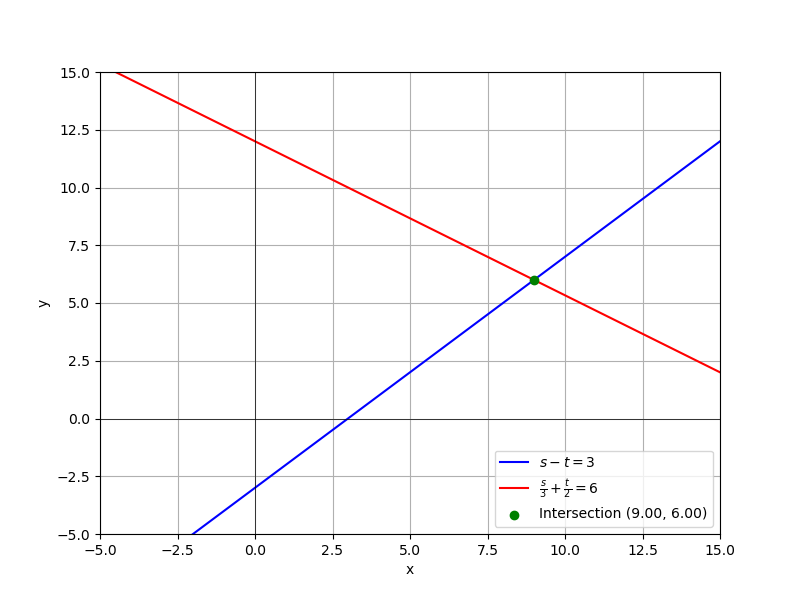
\includegraphics[width=\columnwidth]{figures/Figure_1.png}
	\label{stemplot}
\end{figure}
\end{document}

